\documentclass[british, journal]{IEEEtran}
\usepackage{float}
\usepackage{subfig}
\usepackage{graphicx}
\usepackage{array}
\onecolumn
\begin{document}

\begin{figure}[H]
\begin{centering}
\subfloat
%\label{fig:buck-schematic}Schematic (digital control in analogue environment).
{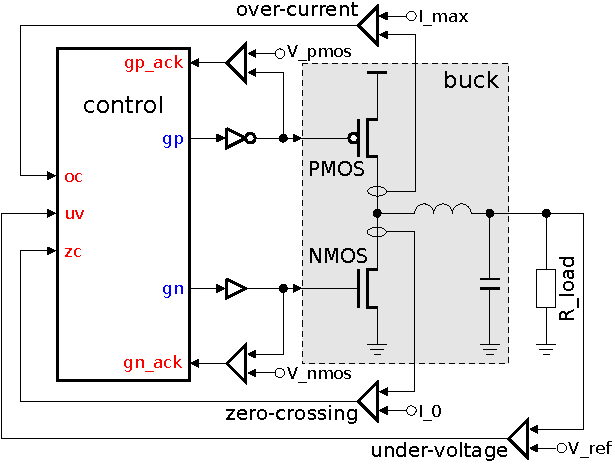
\includegraphics[scale=0.7]{Images/schematic-buck}}
\par
\subfloat
%\label{fig:buck-spec}Informal description of three behavioural scenarios.
{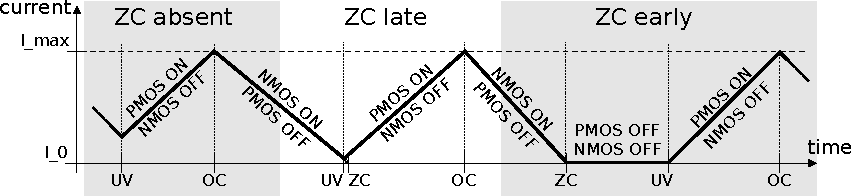
\includegraphics[scale=0.6]{Images/spec-buck}}
\par
\end{centering}
%\protect\caption{\label{fig:buck}Buck converter and its informal description.}
\vspace{-3mm}
\end{figure}

\begin{figure}[H]
	\begin{centering}
		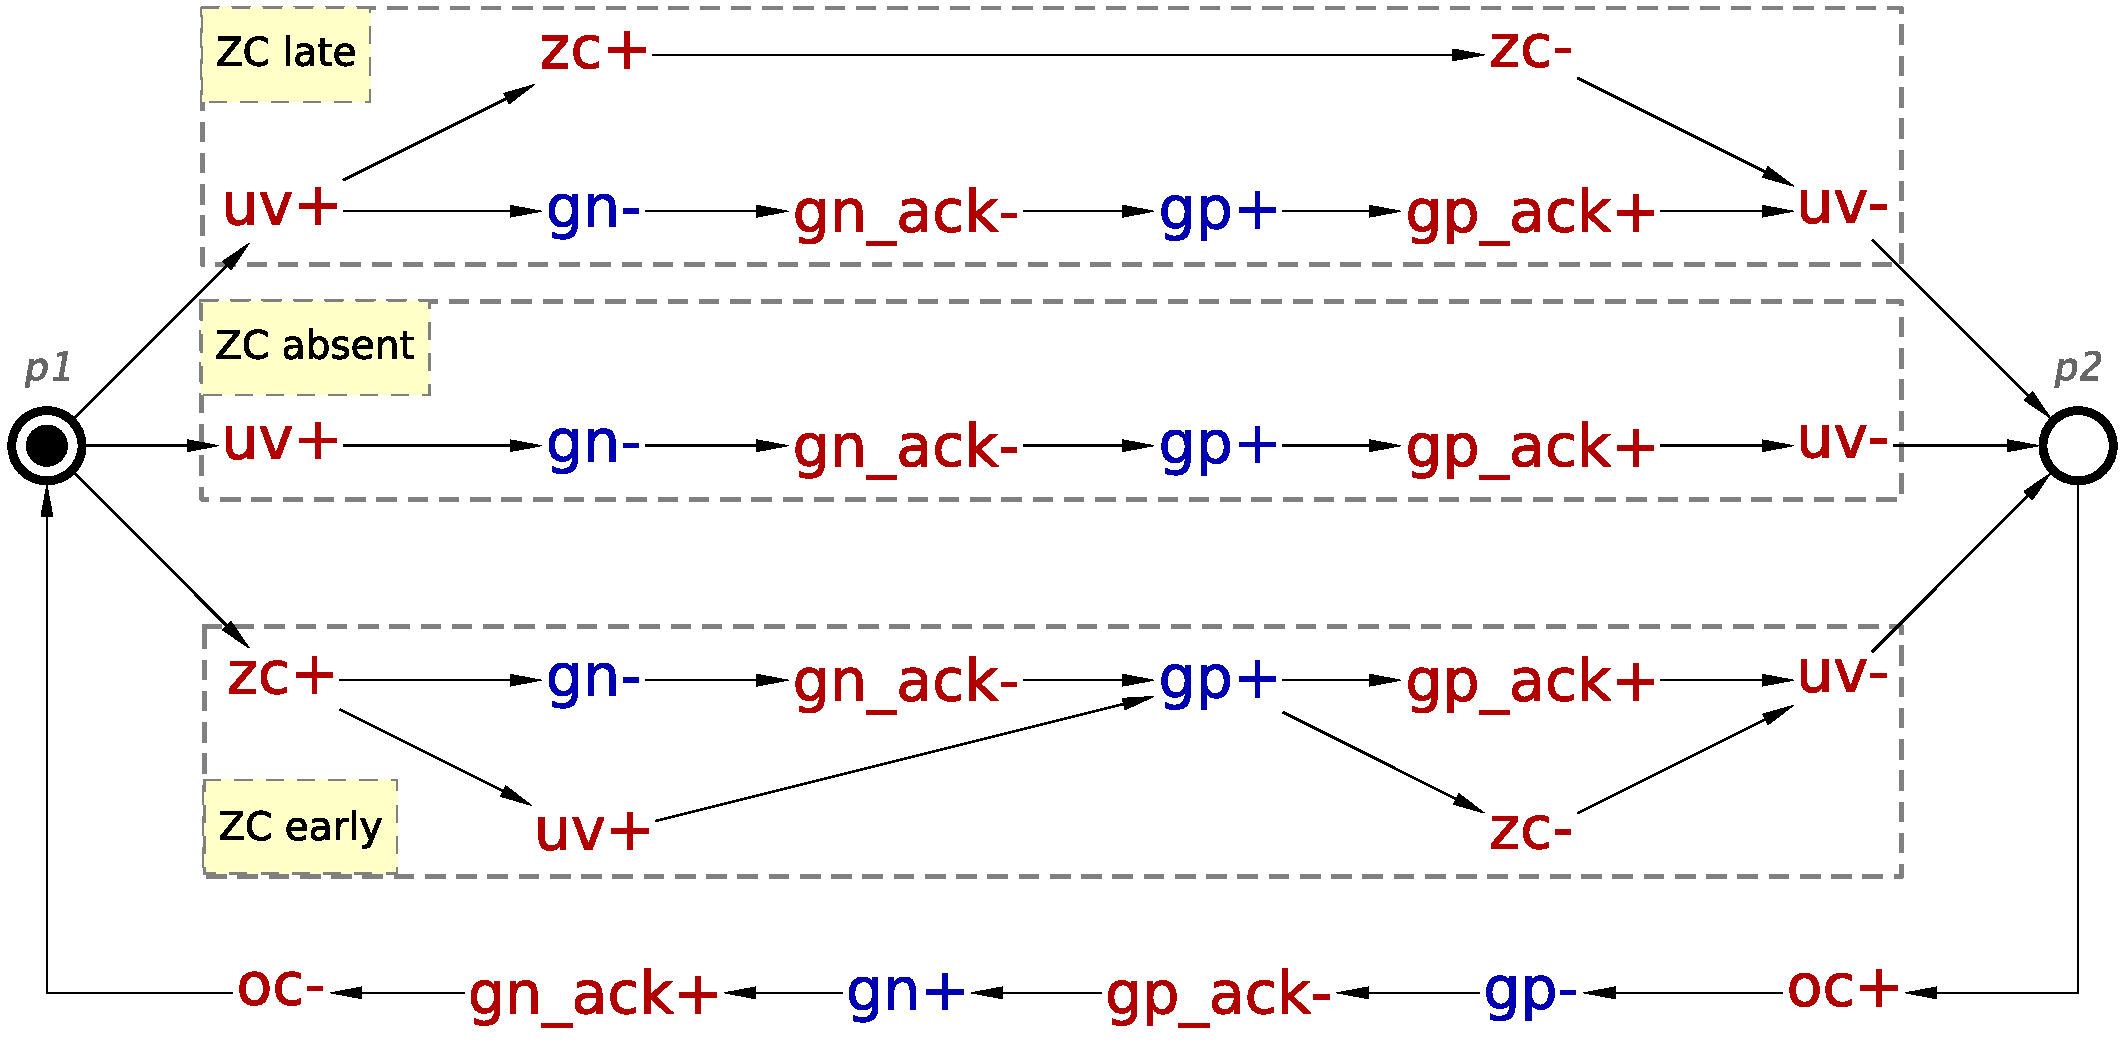
\includegraphics[scale=0.23]{Images/stg-buck}
		\par
%		\protect\caption{\label{fig:Monolithic-buck}STG specification of a simple buck converter.}
		\par\end{centering}
	\vspace{-3mm}
\end{figure}

\begin{figure}[H]
	\begin{centering}
		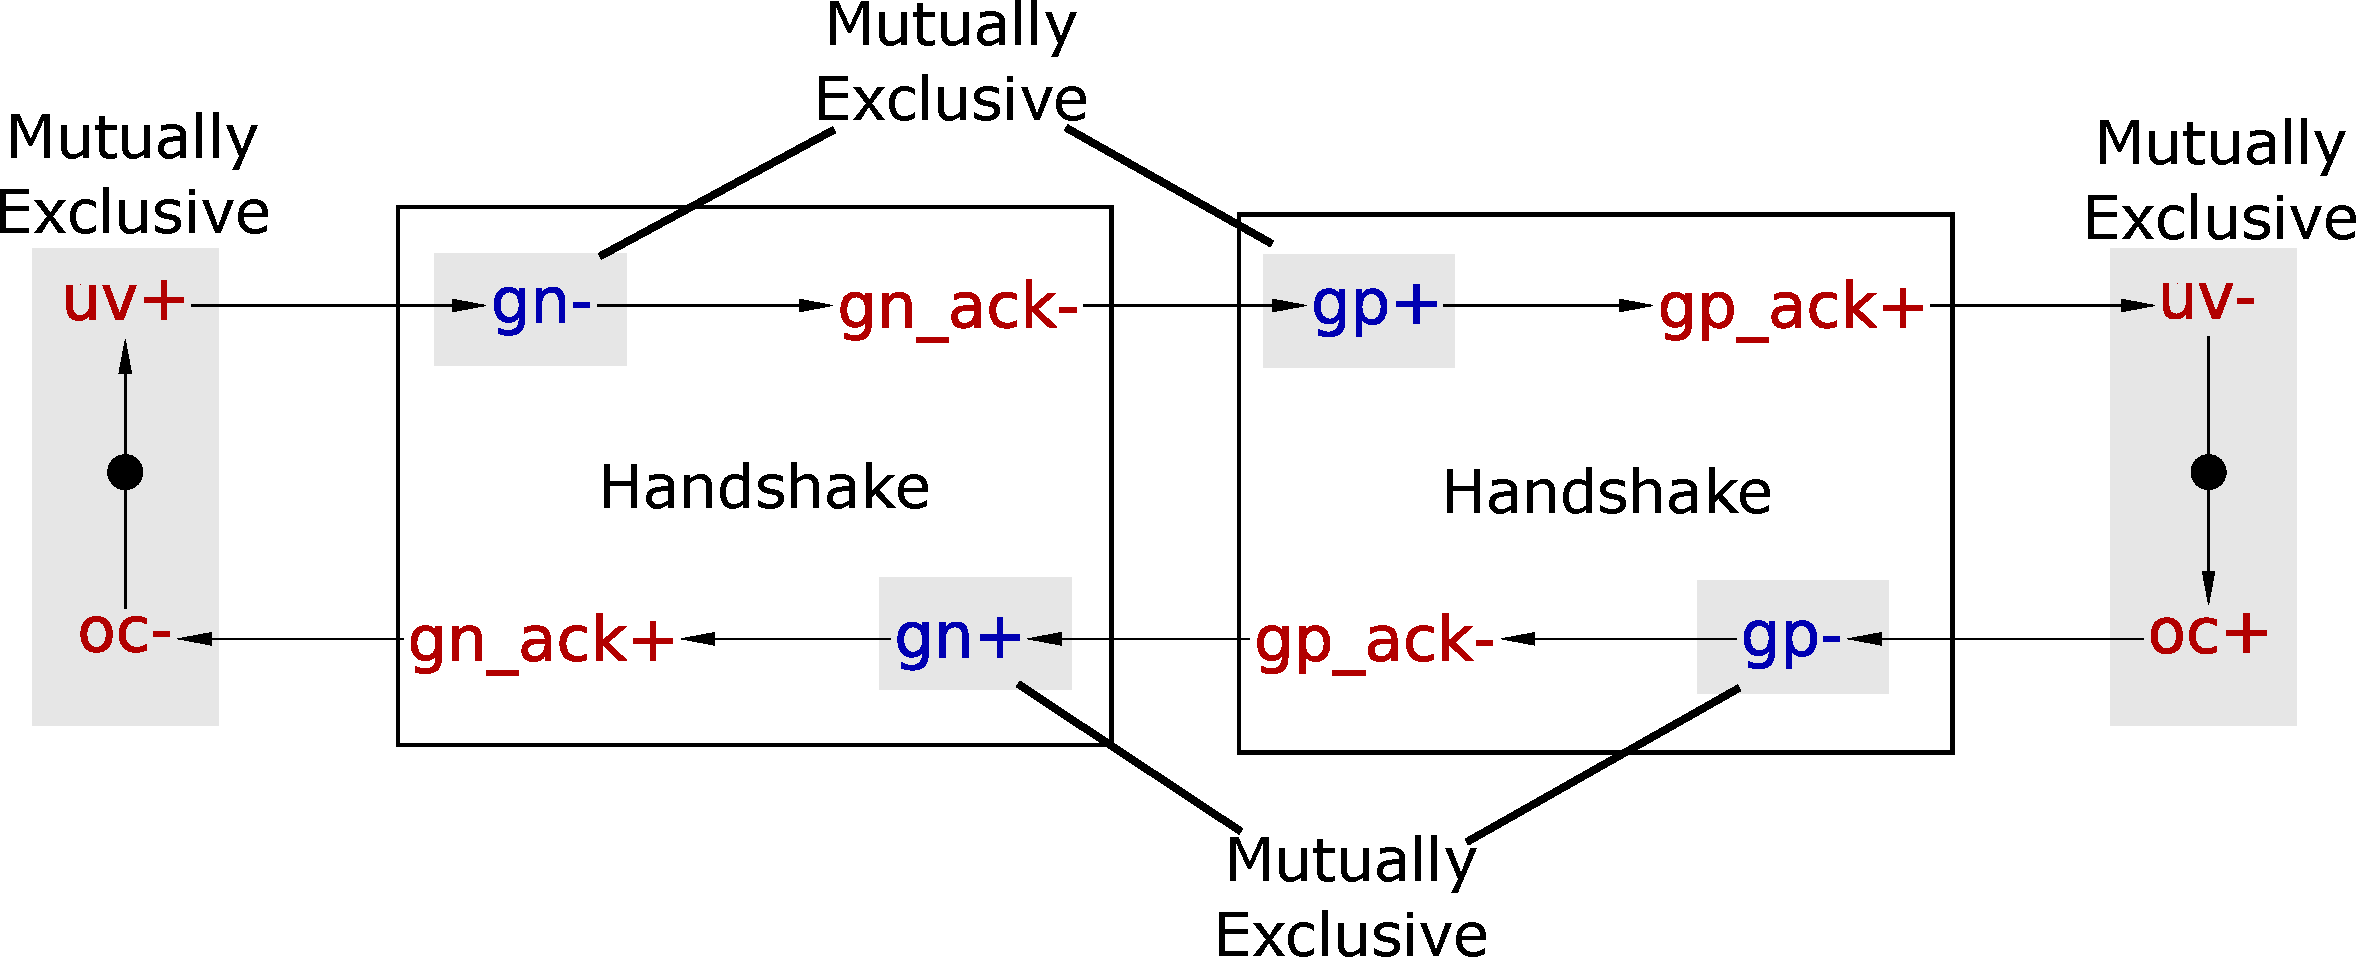
\includegraphics[scale=0.225]{Images/stg-breakdown}
		\par
%		\protect\caption{\label{fig:stg-breakdown}Deconstructing the STG of the ZC absent scenario.}
		\par\end{centering}
	\vspace{-4mm}
\end{figure}

\begin{figure}[H]
	\begin{centering}
		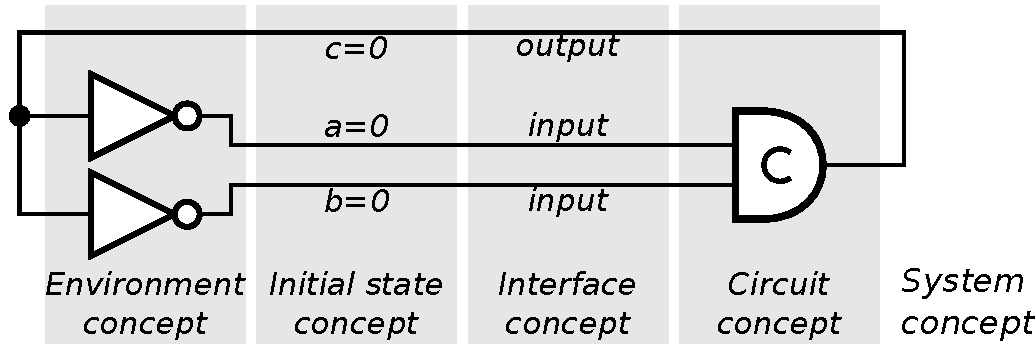
\includegraphics[scale=0.51]{Images/C-element-with-environment}
		\par\end{centering}
%	\protect\caption{\label{fig:cElement-concepts}Example system specified using concepts.}
	\vspace{-3mm}
\end{figure}

\begin{figure}[H]
	\begin{centering}
		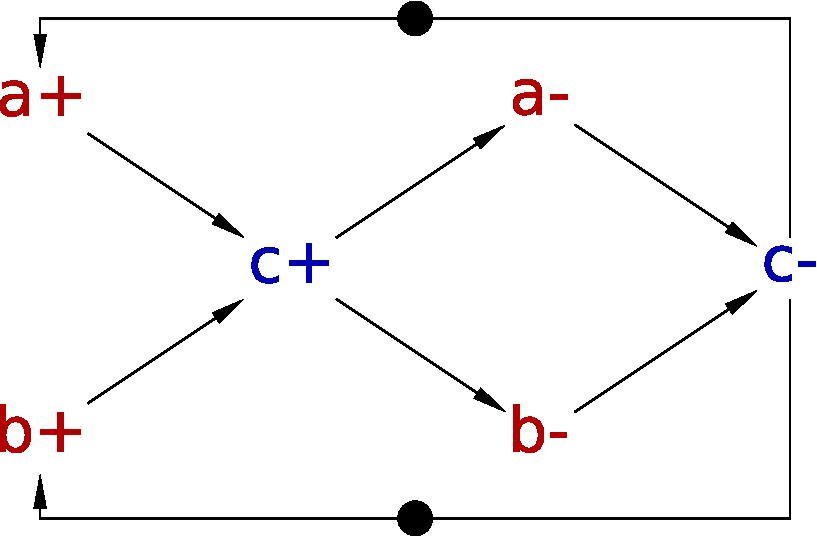
\includegraphics[scale=0.3]{Images/stg-cElement}
		\par\end{centering}
%	\protect\caption{\label{fig:cElement STG composition}STG for the example system.}
	\vspace{-2mm}
\end{figure}

\begin{figure}[H]
	\begin{centering}
		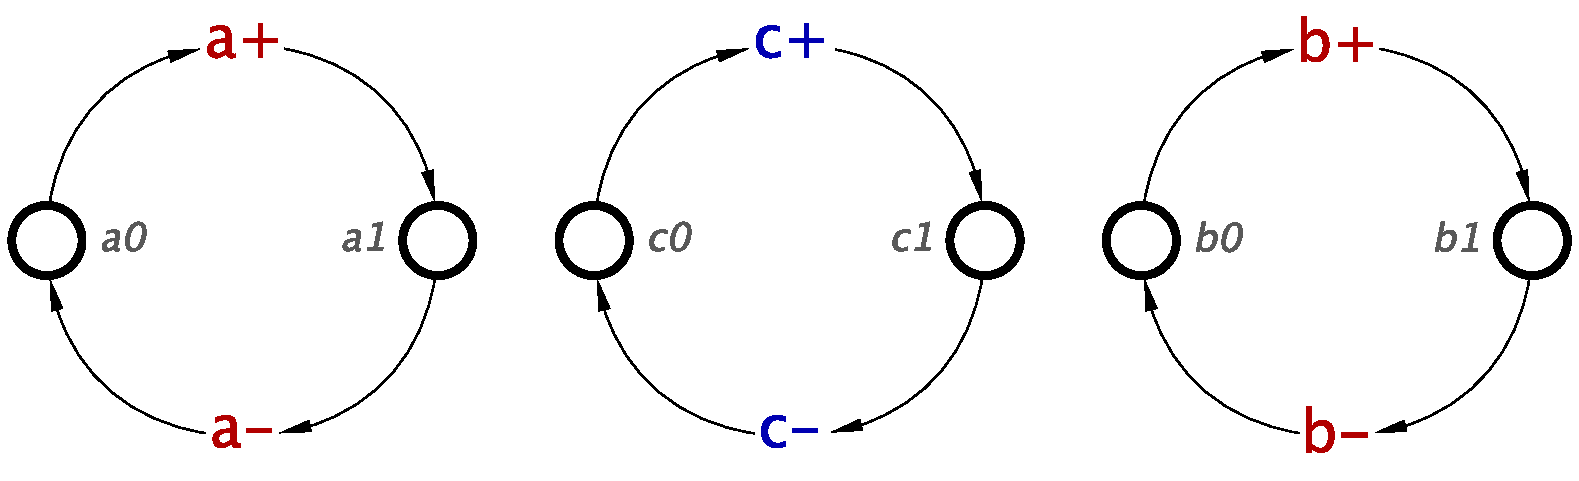
\includegraphics[scale=0.3]{Images/Step-by-step1}
		\par
		\vspace{-2mm}
%		\protect\caption{\label{fig:step-by-step1}The first step: create consistency loops.}
	\end{centering}
	\vspace{-5mm}
\end{figure}

\begin{figure}[H]
	\vspace{-1mm}
	\begin{centering}
		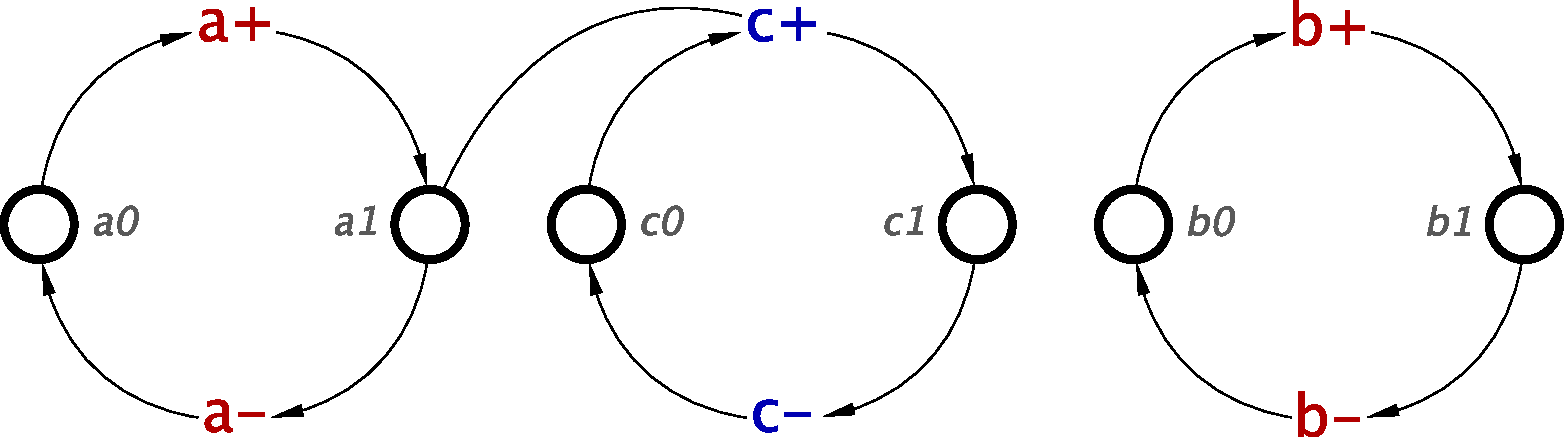
\includegraphics[scale=0.3]{Images/Step-by-step2}
		\par
		\vspace{-1mm}
%		\protect\caption{\label{fig:step-by-step2}The second step: add causality concept $a^{+}\rightsquigarrow c^{+}$.}
	\end{centering}
	\vspace{-1mm}
\end{figure}

\begin{figure}[H]
	\vspace{-1mm}
	\begin{centering}
		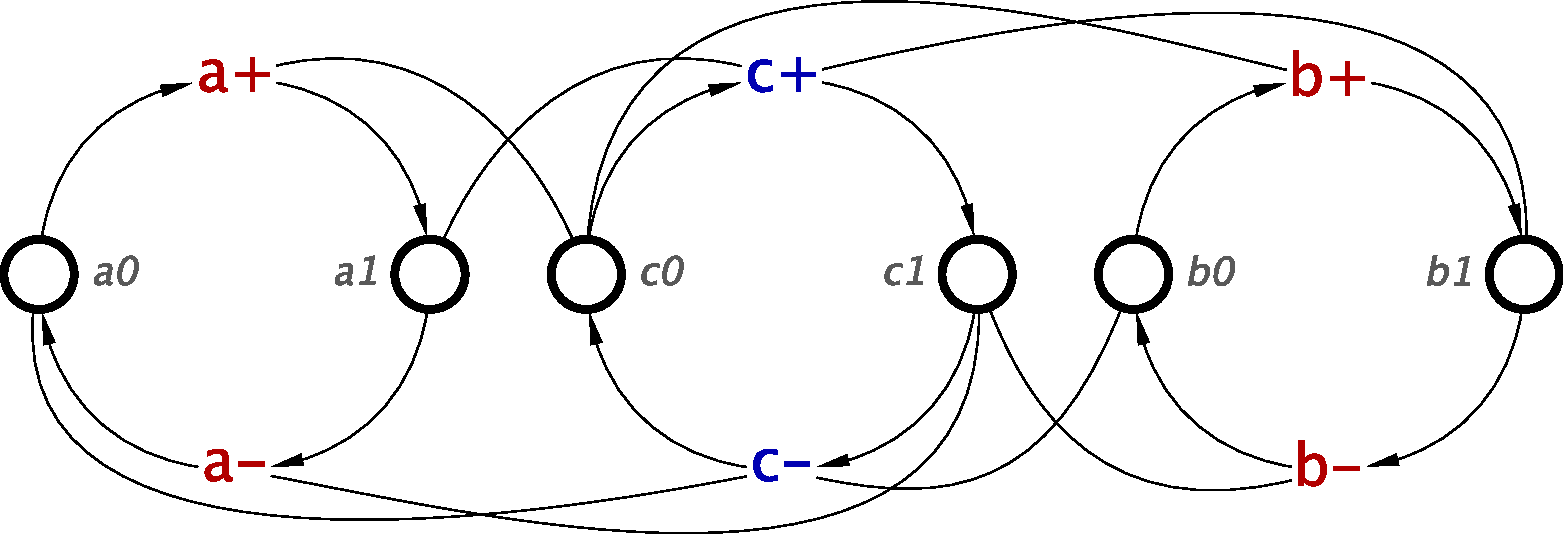
\includegraphics[scale=0.3]{Images/Step-by-step9}
		\par
		\vspace{-1mm}
%		\protect\caption{\label{fig:step-by-step9}Finish the second step: add all causality concepts.}
		\par\end{centering}
	\vspace{-2mm}
\end{figure}

\begin{figure}[H]
	\vspace{-2mm}
	\begin{centering}
		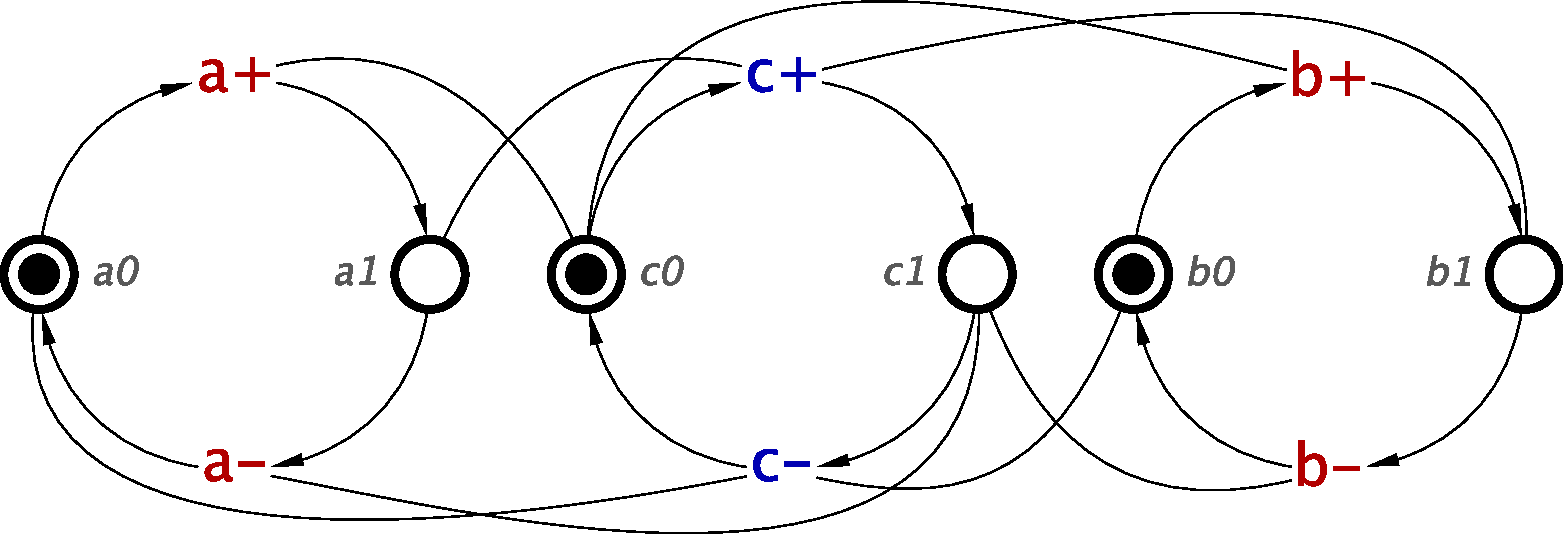
\includegraphics[scale=0.3]{Images/Step-by-step12}
		\par
		\vspace{-1mm}
%		\protect\caption{\label{fig:step-by-step12}The final step: set the initial state.}
		\par\end{centering}
	\vspace{-1mm}
\end{figure}

\begin{figure}[H]
	\begin{centering}
		\subfloat{\begin{centering}
%				\label{fig:cElement}$\mathsf{cElement}(a,b,c)$
				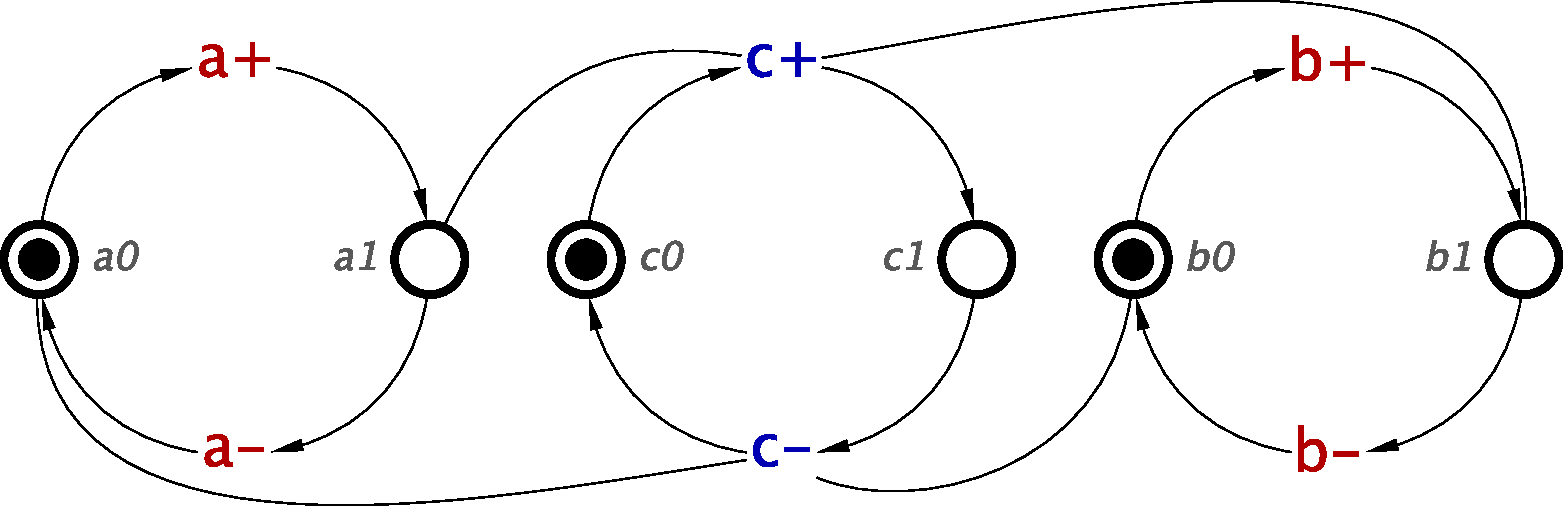
\includegraphics[scale=0.3]{Images/C-element}
				\par\end{centering}
		}
		\par
		\subfloat{\begin{centering}
%				\label{fig:inverterca}$\mathsf{inverter}(c,a)$
				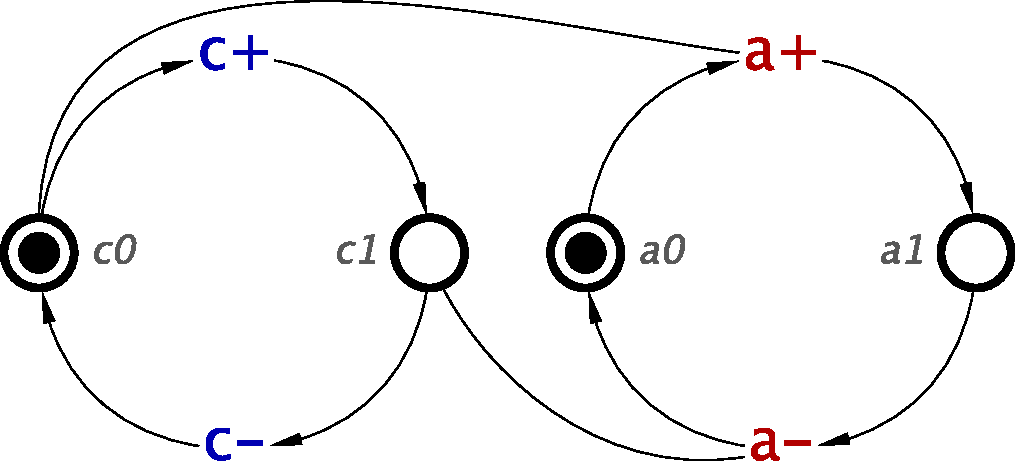
\includegraphics[scale=0.3]{Images/inverter(c,a)}
				\par\end{centering}
			
		}
		\par
		\subfloat{\begin{centering}
%				\label{fig:inverterba} $\mathsf{inverter}(c,b)$
				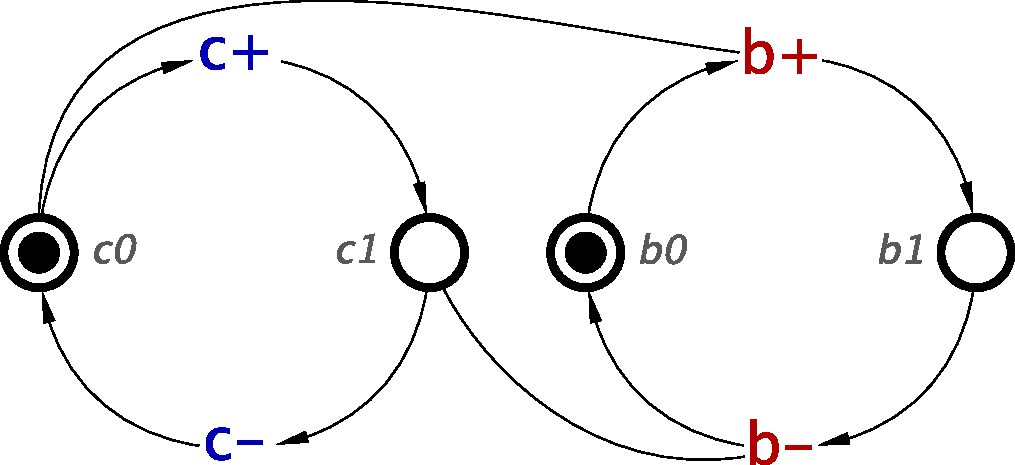
\includegraphics[scale=0.3]{Images/inverter(c,b)}
				\par\end{centering}
		}
		\par\end{centering}
%	\protect\caption{\label{fig:IndividConceptStgs}Partial translation of concepts into STGs}
	\vspace{-6mm}
\end{figure}

\begin{figure*}[H]
	\begin{centering}
		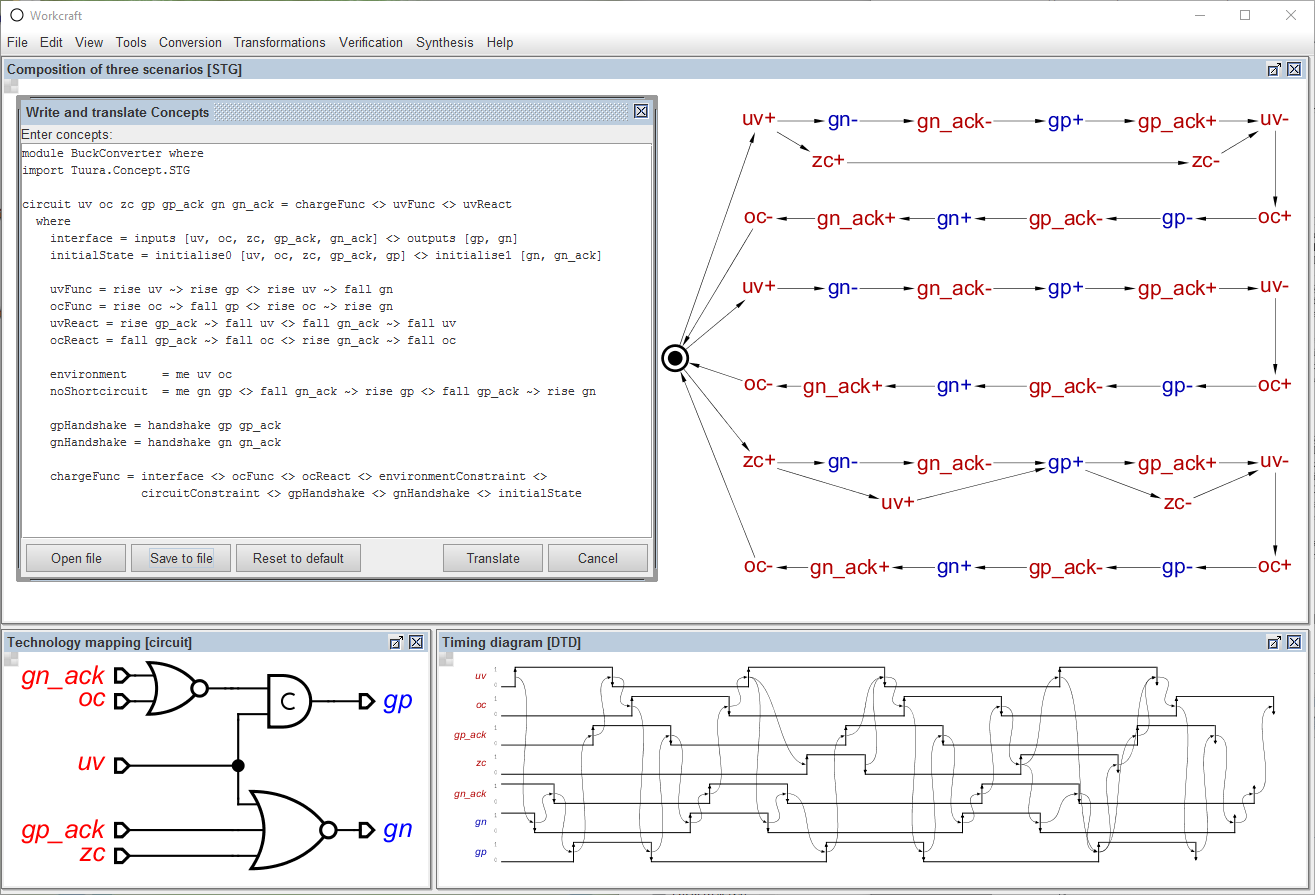
\includegraphics[scale=0.51]{Images/design_flow_wc_screenshot}
		\par\end{centering}
	
%	\protect\caption{\label{fig:workcraft_screenshot}Stages of the design flow when using asynchronous concepts in \noun{Workcraft}.}
	\vspace{-4mm}
\end{figure*}

\begin{figure}[H]
	\begin{centering}
		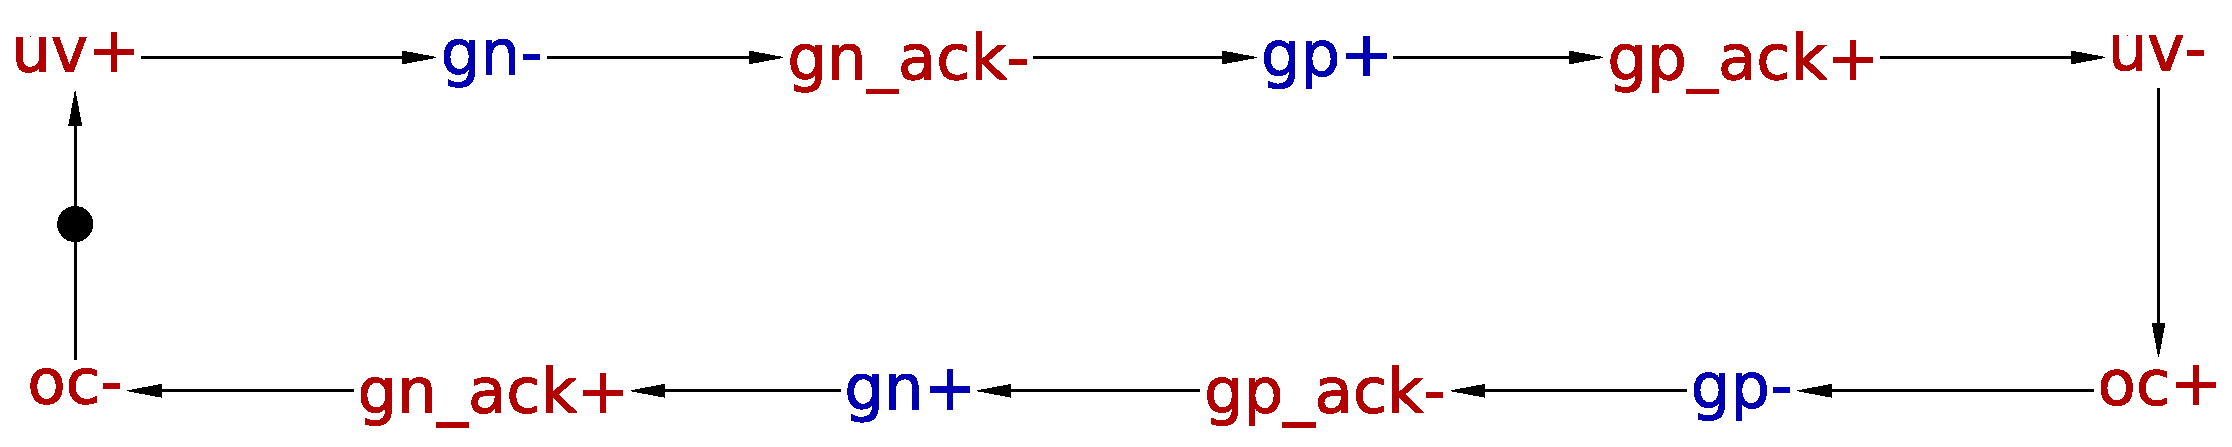
\includegraphics[scale=0.23]{Images/stg-UV_without_ZC}
		\par\end{centering}
%	\protect\caption{\label{fig:zcAbsentScenario STG} STG for the \textsf{zcAbsentScenario} concept.}
	\vspace{-4mm}
\end{figure}

\begin{figure}[H]
	\begin{centering}
		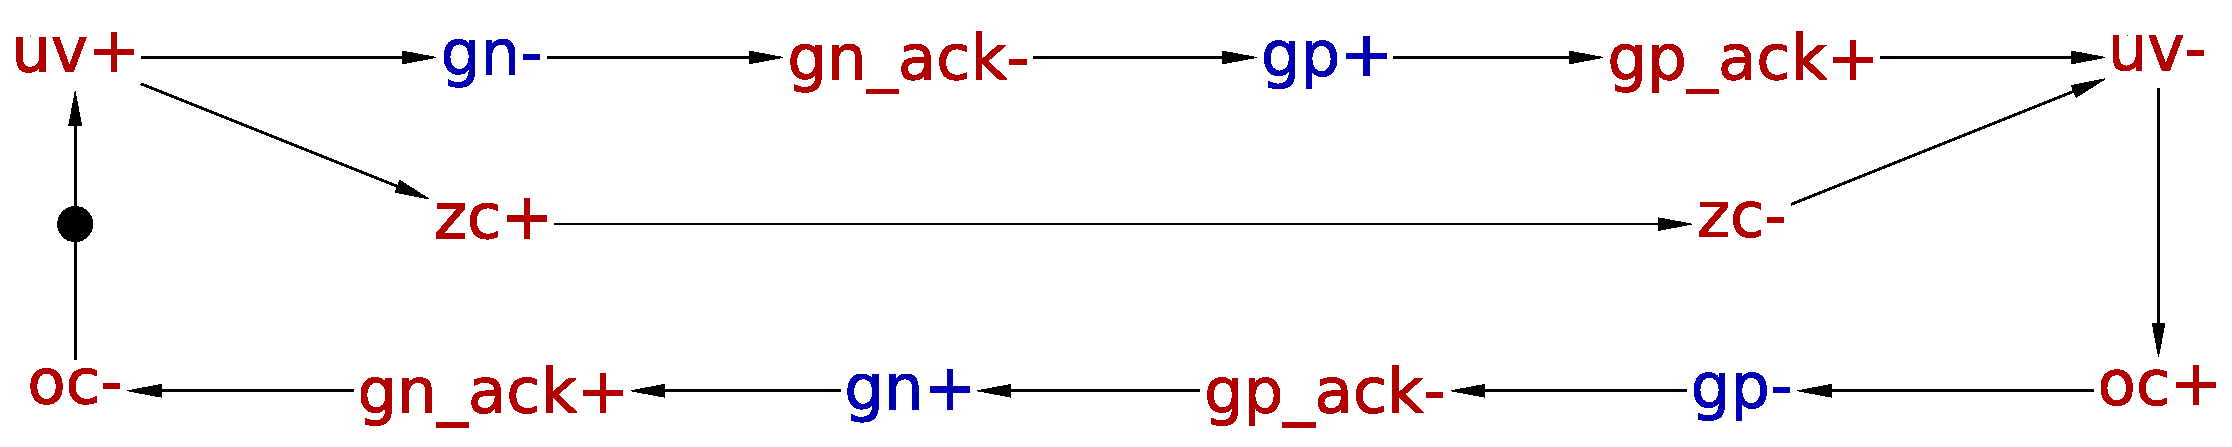
\includegraphics[scale=0.23]{Images/stg-UV_before_ZC}
		\par\end{centering}
%	\protect\caption{\label{fig:zcLateScenario STG}STG for the \textsf{zcLateScenario} concept.}
	\vspace{-4mm}
\end{figure}

\begin{figure}[H]
	\begin{centering}
		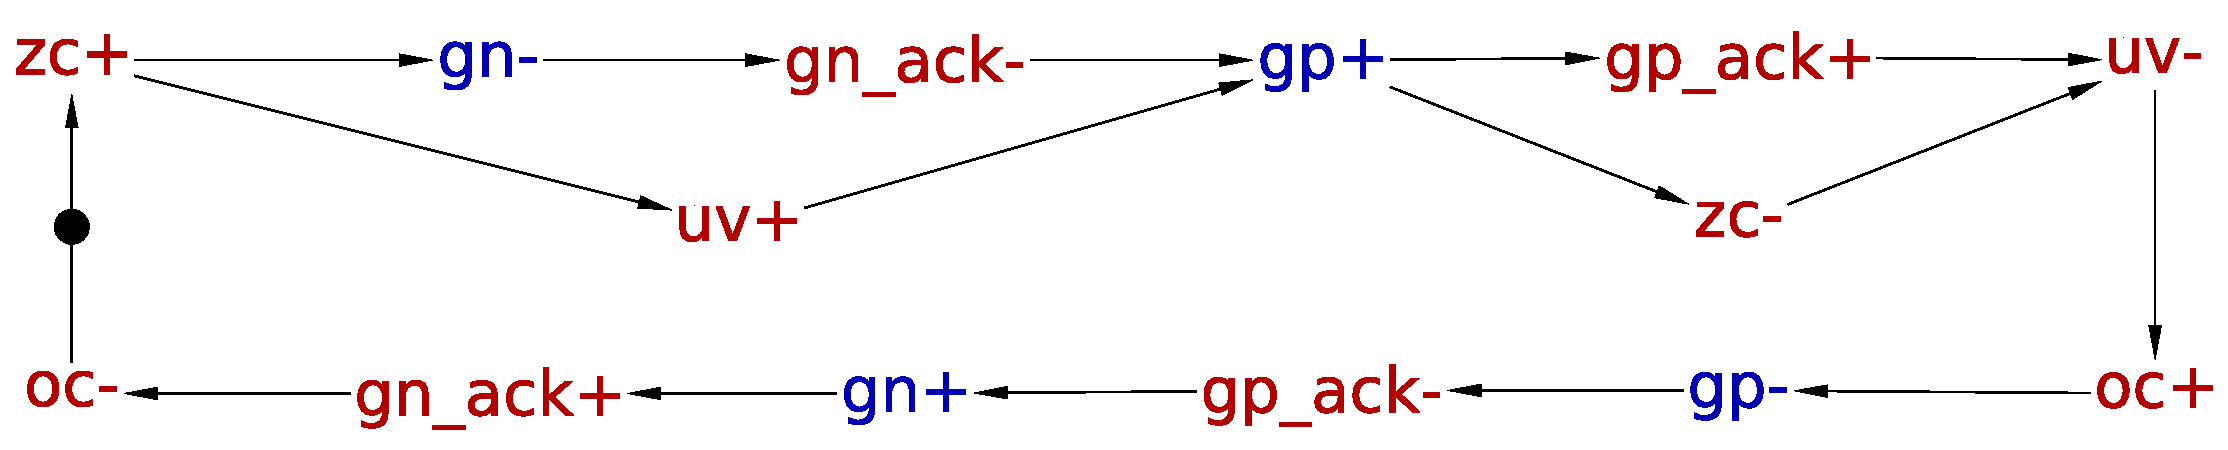
\includegraphics[scale=0.23]{Images/stg-UV_after_ZC}
		\par\end{centering}
%	\protect\caption{\label{fig:zcEarlyScenario STG}STG for the \textsf{zcEarlyScenario} concept.}
	\vspace{-3mm}
\end{figure}

\begin{figure}[H]
	\begin{centering}
		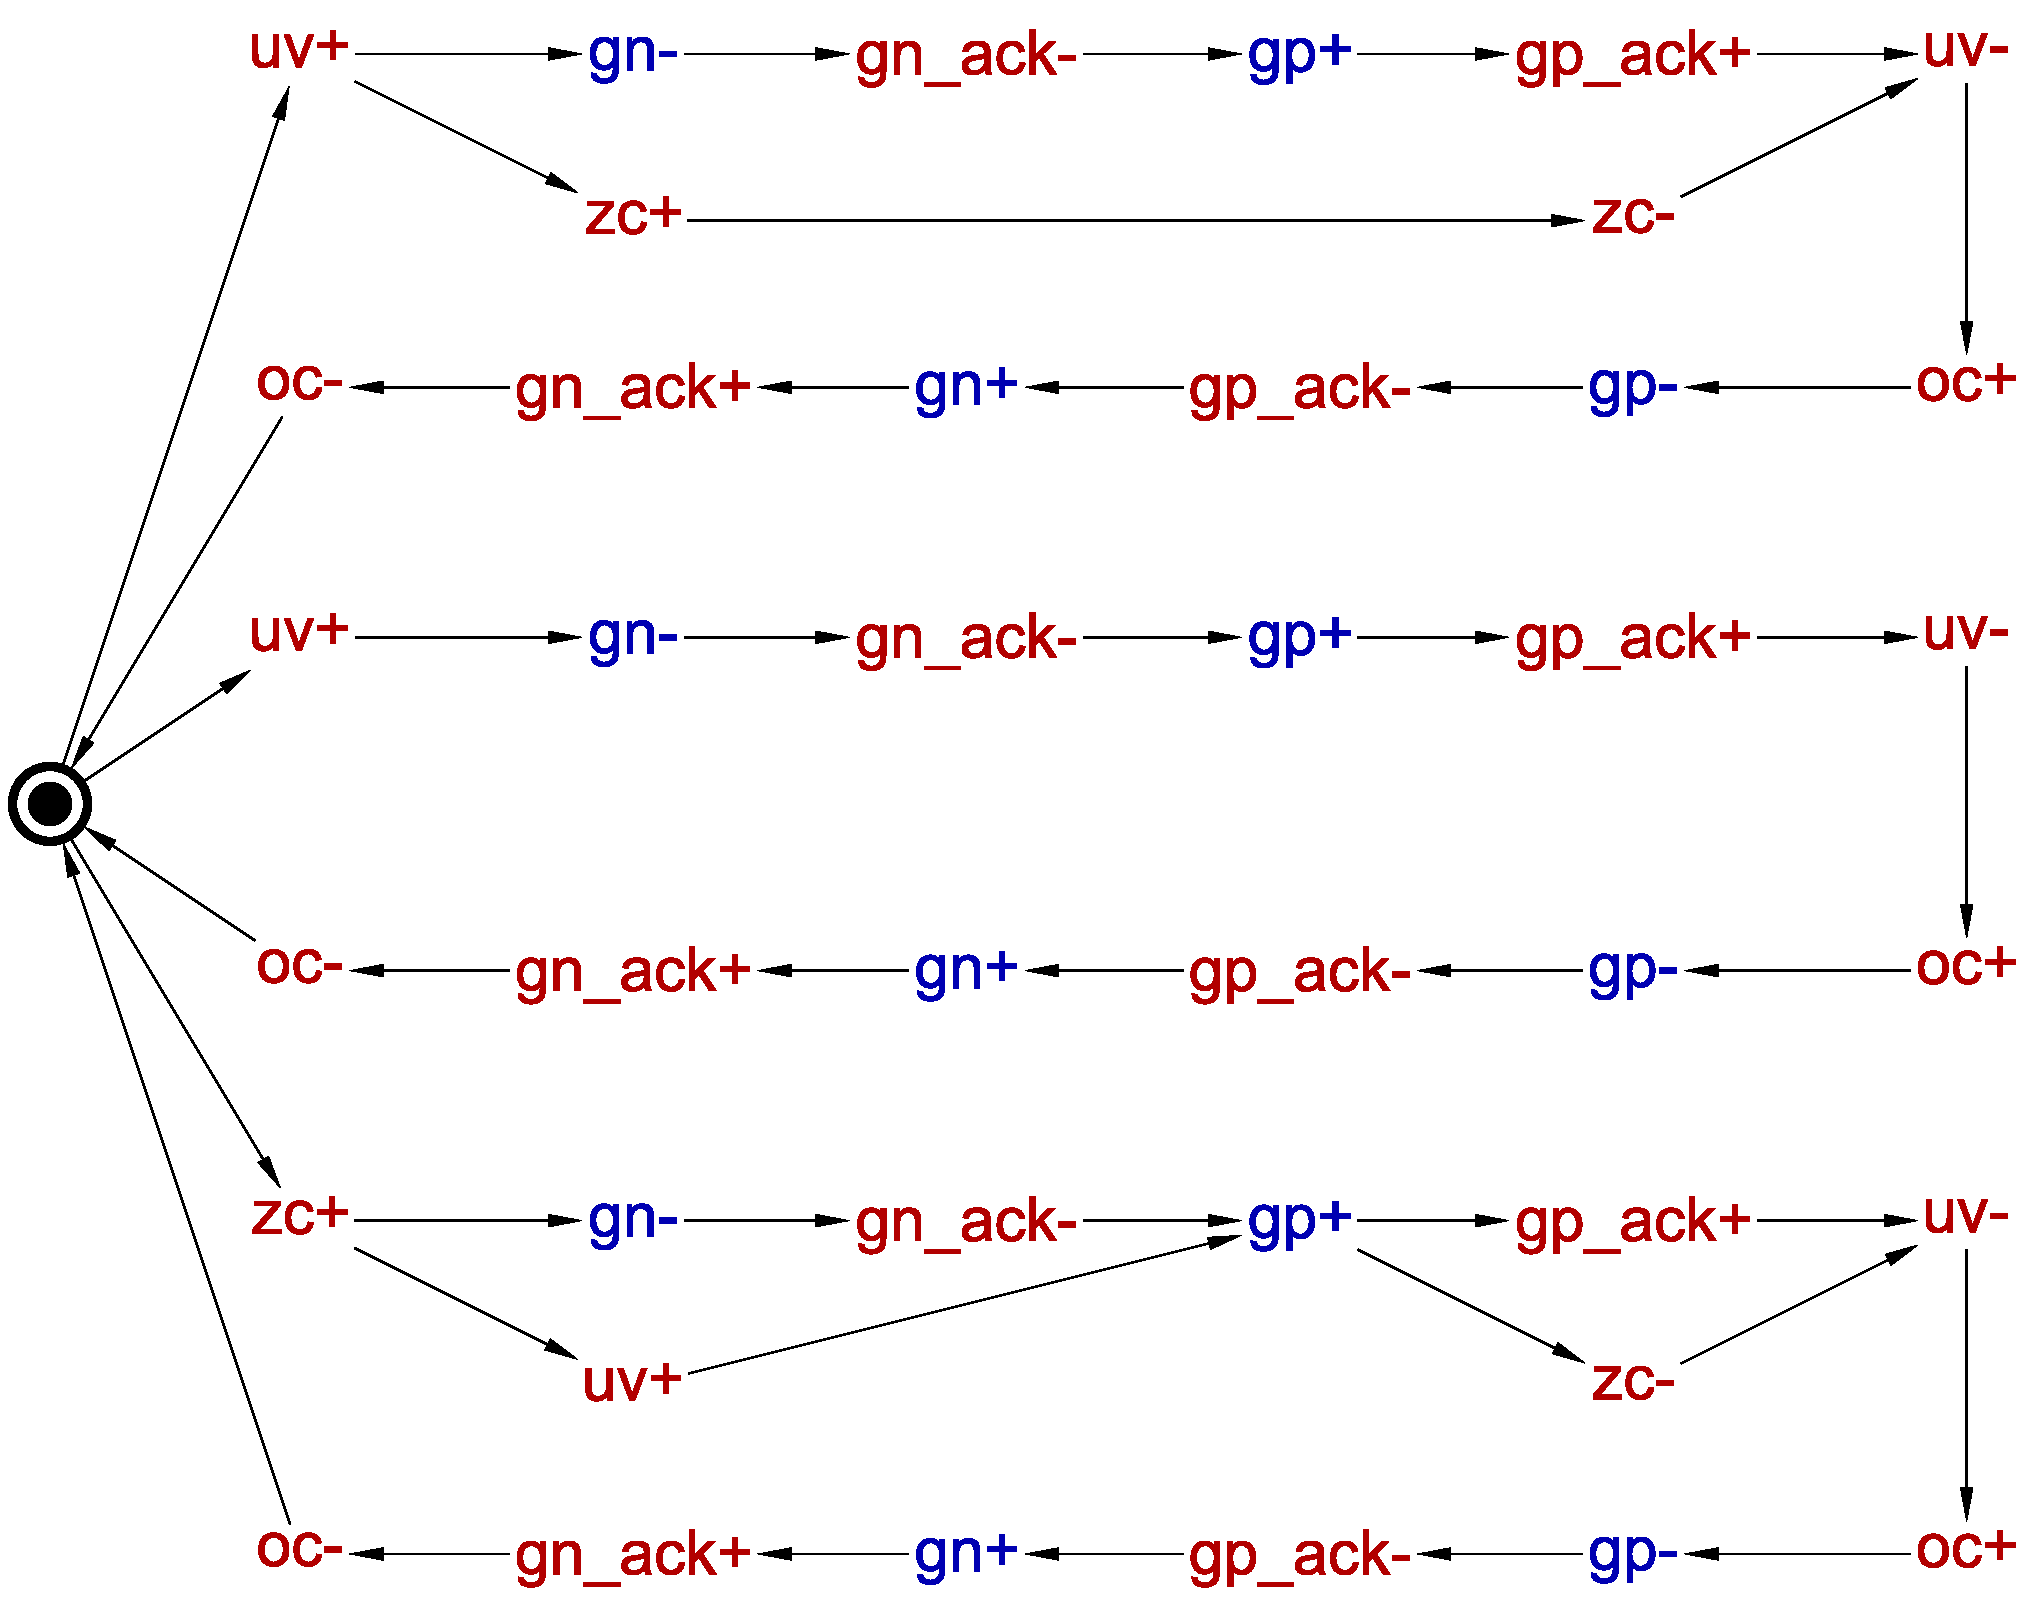
\includegraphics[scale=0.23]{Images/stg-buck-scenarios_merged}
		\par\end{centering}
	\begin{centering}
%		\protect\caption{\label{fig:buck STG}Complete STG for a buck converter.}
		\par\end{centering}
	\vspace{-3mm}
\end{figure}

\begin{figure}[H]
	\begin{centering}
		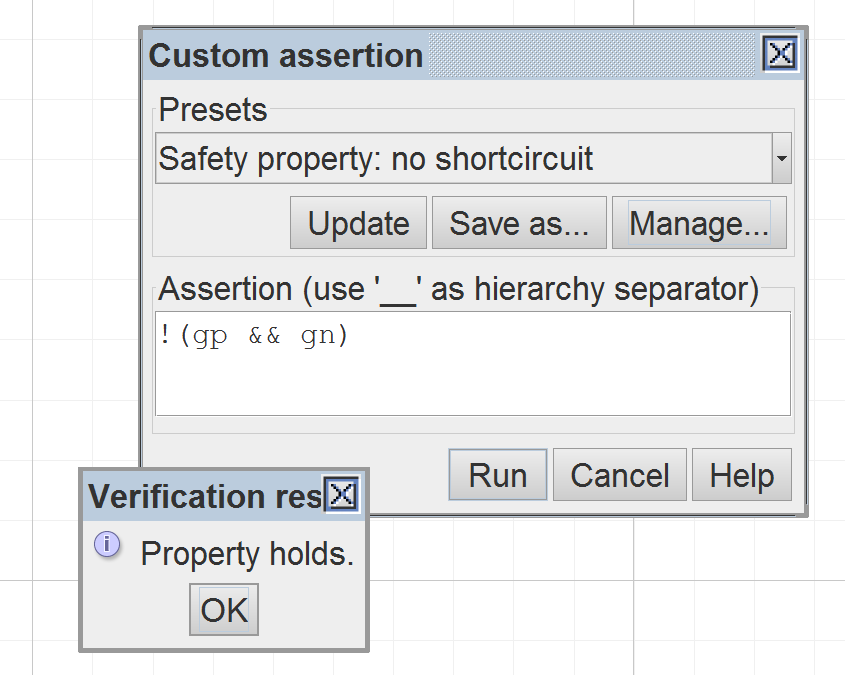
\includegraphics[scale=0.75]{Images/screenshot-custom-assertion}
		\par\end{centering}
	\begin{centering}
%		\protect\caption{\label{fig:custom_assertion}Custom verification of no shortcircuit.}
		\par\end{centering}
	\vspace{-3mm}
\end{figure}

\begin{figure}[H]
	\begin{centering}
		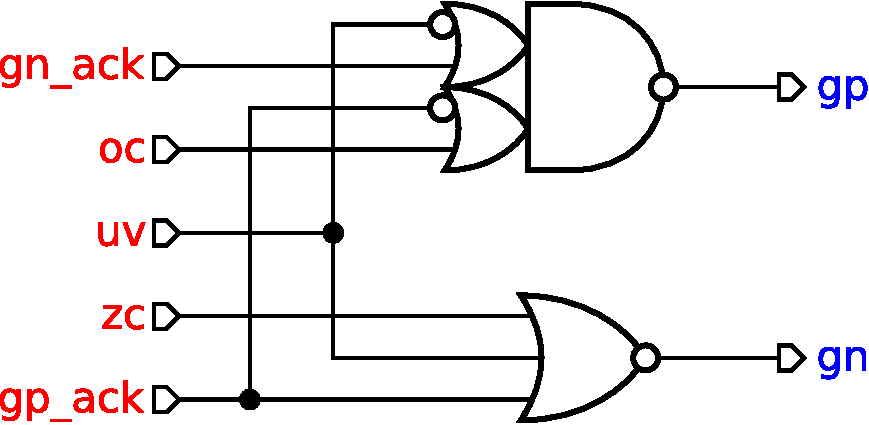
\includegraphics[scale=0.35]{Images/complex-gate-circuit-buck}
		\par\end{centering}
	
%	\protect\caption{\label{fig:complex-gate-circuit}Complex gate implementation.}
\end{figure}

\begin{figure}[H]
	\begin{centering}
		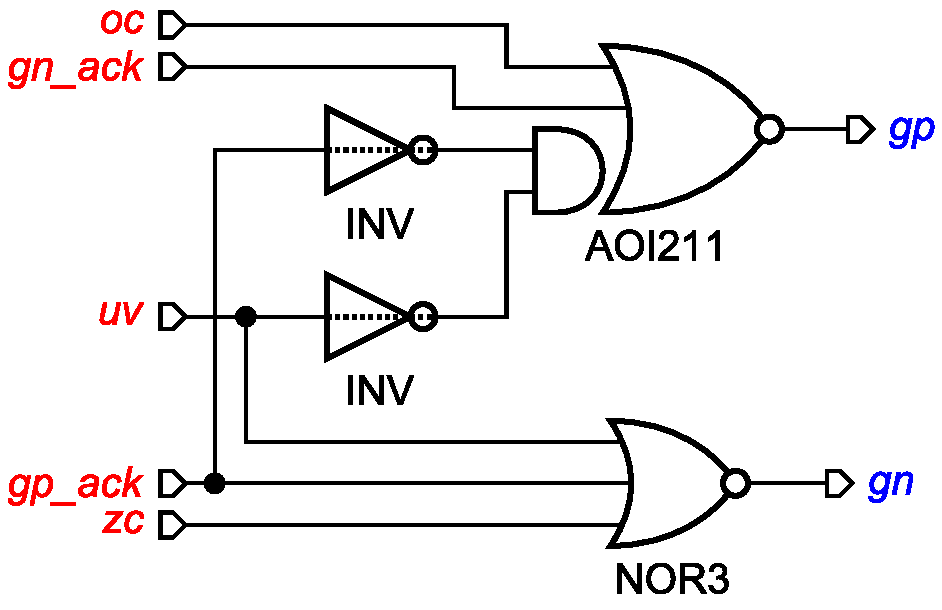
\includegraphics[scale=0.35]{Images/circuit-buck-mapped-pfy-wc.pdf}
		\par\end{centering}
	
%	\protect\caption{\label{fig:tech-mapped-circuit}Technology mapped implementation.}
\end{figure}

\begin{figure}[H]
	\begin{centering}
		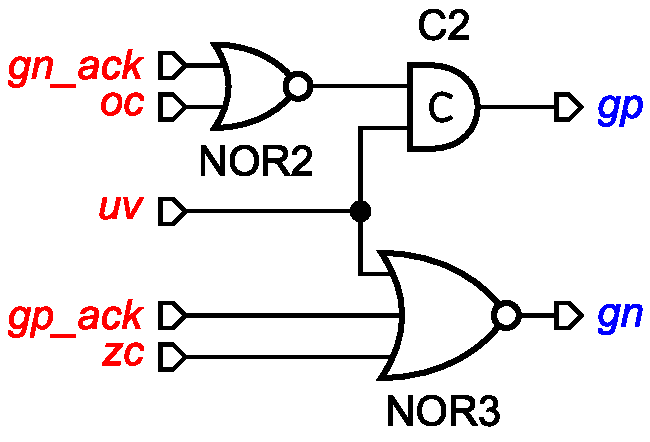
\includegraphics[scale=0.35]{Images/circuit-buck-deco2-wc}
		\par\end{centering}
%	\protect\caption{\label{fig:circuit-buck-deco2}Technology mapping into 2-input gates/latches.}
\end{figure}

\begin{table*}[h]
%	\caption{A comparison of features of related work and the proposed method \label{tab:related_work}}
	\centering
	\begin{tabular}[htb]{| m{2.6cm} | m{2.0cm} | m{1.3cm} | m{1.5cm} | m{1.5cm} | m{1.7cm} | m{1.9cm} |}
		\hline
		Method             & \,Asynchronous support & \,Tool support  & \,Gate-level & \,Event-level & \,Protocol-level  & \,Design focus \\ \hline \hline
		Concepts            & Yes                               & Yes                       & Yes                       & Yes                         & Yes                              & Little digital \\ \hline
		Balsa             & Yes                               & Yes                        & Yes                       & No                          & Yes                              & Big digital \\ \hline
		Biscotti            & Yes                               & Yes                         & Yes                       & No                          & No                               & Big digital \\ \hline
		Lava              & No                               & Yes                       & Yes                       & No                          & Yes                              & Big digital \\ \hline
		C$\lambda$ash     & No                               & Yes                        & Yes                       & No                          & Yes                              & Big digital \\ \hline
		Snippets          & No                                & No                        & No                        & No                          & No                               & Little digital \\ \hline
		DI algebra        & Yes                               & No                         & No                        & Yes                         & No                               & Little digital \\ \hline
		Structural design & No                                & Yes                        & No                        & No                          & No                               & Modular \\ \hline
	\end{tabular}
	\vspace{-3mm}
\end{table*}

\end{document}
